% Autor: Simon May
% Datum: 2017-10-05
% Diese Datei bietet ein minimalistisches Grundgerüst für ein LaTeX-Dokument,
% z.B. für die Bearbeitung der Aufgaben.
\documentclass[
	% Papierformat
	a4paper,
	% Schriftgröße (beliebige Größen mit „fontsize=Xpt“)
	12pt,
	% Schreibt die Papiergröße korrekt ins Ausgabedokument
	pagesize,
	% Sprache für z.B. Babel
	ngerman
]{scrartcl}

% Achtung: Die Reihenfolge der Pakete kann (leider) wichtig sein!
% Insbesondere sollten (so wie hier) babel, fontenc und inputenc (in dieser
% Reihenfolge) als Erstes und hyperref und cleveref (Reihenfolge auch hier
% beachten) als Letztes geladen werden!

% Silbentrennung etc.; Sprache wird durch Option bei \documentclass festgelegt
\usepackage{babel}
% Verwendung der Zeichentabelle T1 (Sonderzeichen etc.)
\usepackage[T1]{fontenc}
% Legt die Zeichenkodierung der Eingabedatei fest, z.B. UTF-8
\usepackage[utf8]{inputenc}
% Schriftart
\usepackage{lmodern}
% Zusätzliche Sonderzeichen
\usepackage{textcomp}

% Mathepaket (intlimits: Grenzen über/unter Integralzeichen)
\usepackage[intlimits]{amsmath}
% Ermöglicht die Nutzung von \SI{Zahl}{Einheit} u.a.
\usepackage{siunitx}
% Zum flexiblen Einbinden von Grafiken (\includegraphics)
\usepackage{graphicx}
% Abbildungen im Fließtext
\usepackage{wrapfig}
% Abbildungen nebeneinander (subfigure, subtable)
\usepackage{subcaption}
% Funktionen für Anführungszeichen
\usepackage{csquotes}
% Zitieren, Bibliographie
\usepackage{biblatex}


% Verlinkt Textstellen im PDF-Dokument
\usepackage[unicode]{hyperref}
% "Schlaue" Referenzen (nach hyperref laden!)
\usepackage{cleveref}

% siunitx: Deutsche Ausgabe, Messfehler getrennt mit ± ausgeben
\sisetup{
	locale=DE,
	separate-uncertainty
}

 


\begin{document}
\begin{titlepage}
	\centering
	{\scshape\LARGE Versuchsbericht zu \par}
	\vspace{1cm}
	{\scshape\huge Raster-Tunnel-Mikroskopie, Spitzenpräparation und Messungen an Graphit und Gold     \par}
	\vspace{2.5cm}
	{\LARGE Gruppe 6 Mo\par}
	\vspace{0.5cm}
	{\large Nils Kulawiak (E-Mail: n\_kula01@wwu.de) \par}
	{\large Oliver Brune (E-Mail: o\_brun02@wwu.de) \par}
	{\large Anthony Pietz (E-Mail: a\_piet09@wwu.de) \par}
	\vfill
	durchgeführt am 17.12.2018\par
	
	\vfill
	betreut von Alexander Timmer\par
	
	\vfill
	{\large \today\par}
\end{titlepage}

\tableofcontents
\newpage

\section{Methode}
Der Stickstofflaser besteht aus zwei gleich geladenen Platten,die über einen Widerstand verbunden sind, und einer Funkenstrecke. Die beiden Platten liegen auf einer leitenden, geerdeten Unterlage, sind jedoch durch eine Folie davon isoliert und funktionieren damit als Elektroden. Zunächst haben die beiden Platten durch Aufladen das gleiche Potential, durch eine Entladung auf die Funkenstrecke entlädt sich eine der beiden Platten schlagartig, was zu einer großen Potentialdifferenz führt. Dadurch kommt es zu einer weiteren Entladung zwischen den beiden Platten an der Stelle an der sie sich am nächsten sind, wodurch es zu einem Zusammenstoß mit den Stickstoffmolekülen kommt. Deshalb werden die Stickstoffmoleküle angeregt und senden durch hauptsächlich spontane Emission Photonen aus. %bin ich mir nicht ganz sicher nochmal überprüfen pls%

Für die ersten 3 Messungen von Pulsenergie, Repetitionsrate und Impulsdauer sind einfache Messungen mit einer Photodiode, die an einem Oszilloskop angeschlossen ist, nötig. Die ersten beiden Messungen werden, dabei mit einer "langsameren" Diode gemessen, während für die letztere die schnelle Diode zu benutzten ist.

\section{Ergebnis}
Zuerst wird versucht die Pulsenergie des Lasers zu bestimmen. Dazu muss zuerst die niedrigste Spannung ermittelt werden. Dazu wird einfach der niedrigste Weert aus \cref{Energie} genommen. 

\begin{figure}[h!]
	\centering
	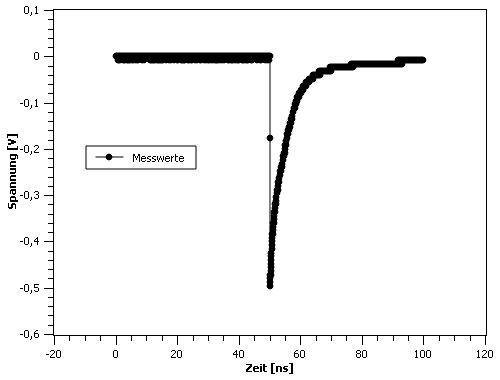
\includegraphics[scale=0.7]{Energie.png}
	\caption{Puls zur Berechnung der Energie}
	\label{Energie}
\end{figure}

Über die Formel
\begin{equation}
E_{p} = \dfrac{1 \mu J}{50mV}U_{min} = \SI{9,92 \pm 0,30}{J}
\end{equation}
lässt sich dann die Energie des Pulses bestimmen.

Daraufhin soll die Repetitionsrate des Lasers bestimmt werden. Dazu wurden mehrere Pulse in \cref{Rep} aufgenommen und jeweils der Abstand zwischen ihnen bestimmt. Dazu wird jeweils der größte Zeitpunkt gewählt an dem der Puls noch messbar ist und dann die Differenz gebildet. Aus dem Mittelwert ergibt sich eine Repetitionsrate von $t_{Rep}$ = $\SI{0,0814 \pm 0,0006}{s]}$, was einer Frequenz von f = $\SI{12,29 \pm 0,09}{Hz}$ entspricht. Das stimmt auch mit dem vom Oszilloskop abgelesenen Wert von f = $\SI{12,15}{Hz}$ überein.

\begin{figure}[h!]
	\centering
	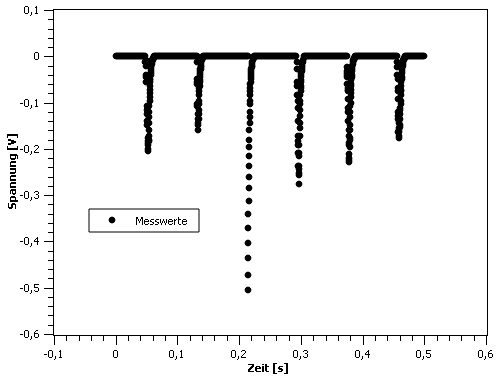
\includegraphics[scale=0.7]{Rep.png}
	\caption{Mehrere Pulse zur Bestimmung der Repetitionsrate}
	\label{Rep}
\end{figure}


Als nächstes soll die Impulsdauer eines einzelnen Impulses bestimmt werden. Dies wird mithilfe von \cref{Pulsdauer} versucht. Die Halbwertsdauer lässt sich relativ einfach bestimmen. Dazu wird einfach geschaut, ab wann die Spannung auf die Hälfte des Maximalwertes abfällt. Daraus ergibt sich eine Halbwertsdauer von $t_{\dfrac{1}{2}} = \SI{13,3 \pm 0,6}{ns}$. Schwieriger ist es die Gesamtdauer des Pulses zu bestimmen, da die Spannung für kleine Werte anfängt zu schwanken. Wenn die Gesamtdauer so definiert ist, dass der Puls zu Ende ist, sobald die Spannung unter 0,24V fällt, dann ergibt sich eine Dauer des Gesamtimpulses von $t = \SI{14,180 \pm 0,0014}{ns}$. Die Definition wurde so gewählt, da ab diesem Wert die Spannung anfangen hat stark zu schwanken, allerdings ist diese Definition relativ willkürlich gewählt. 

\begin{figure}[h!]
	\centering
	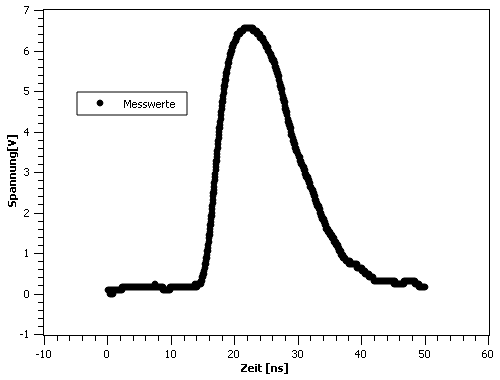
\includegraphics[scale=0.7]{Pulsdauer.png}
	\caption{Genau Auflösung eines Pulses zur Bestimmung der Pulsdauer}
	\label{Pulsdauer}
\end{figure}

\end{document}